\documentclass[12pt, a4paper, twoside]{article}
\usepackage[utf8]{inputenc}
\usepackage[cm]{fullpage}
\usepackage{fancyhdr}
\usepackage{textcomp}
\usepackage{graphicx}
\usepackage{commath}
\usepackage[portuguese]{babel}

\begin{document}

\title{Pré-relatório 1 do Laboratório de Dispositivos e Circuitos Eletrônicos}
\author{Cristiano Silva Júnior: 13/0070629}
\date{\today}
\maketitle

Neste pré-relatório, consideraremos um amplificador operacional (\textit{amp op}) ideal como o do modelo da figura 1.

\begin{figure}
    \centering
    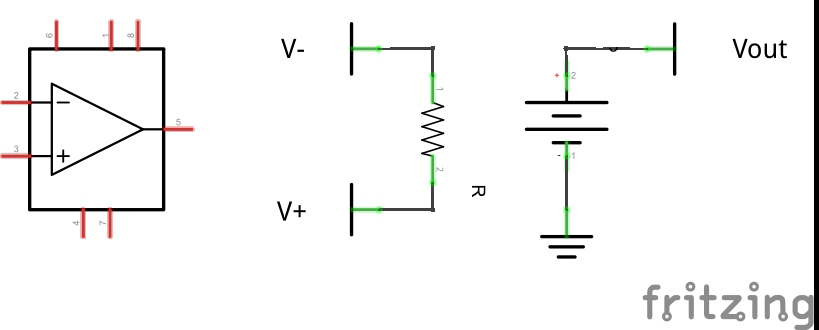
\includegraphics[width=0.8\textwidth]{figs/ex0.jpg}
    \caption{Modelo do amplificador operacional}
\end{figure}

Consideramos, neste modelo, que
$$ V_{out}(s) = \frac{A_0}{1 + s \omega_b} (V_+(s) - V_-(s)) $$
e que
$$ R = \infty $$
para ganhos DC, $A_0=\infty$

\section{Exercício 1}

Tomando como base a família de \textit{amp ops TL074} da \textit{Texas Instruments}, podemos determinar a largura de banda e o \textit{slew rate} pelo \textit{datasheet}. Tomando como base o modelo \textit{TL074A}:

\begin{itemize}
    \item \textit{Bandwidth}: $3MHz$ típico a $25^oC$.
    \item \textit{Slew rate}: $13 V/\mu s$ típico a $25^oC$. \textit{Amp op} montado com alimentação $30V_{pp}$.
\end{itemize}

\section{Exercício 2}

\begin{figure}
    \centering
    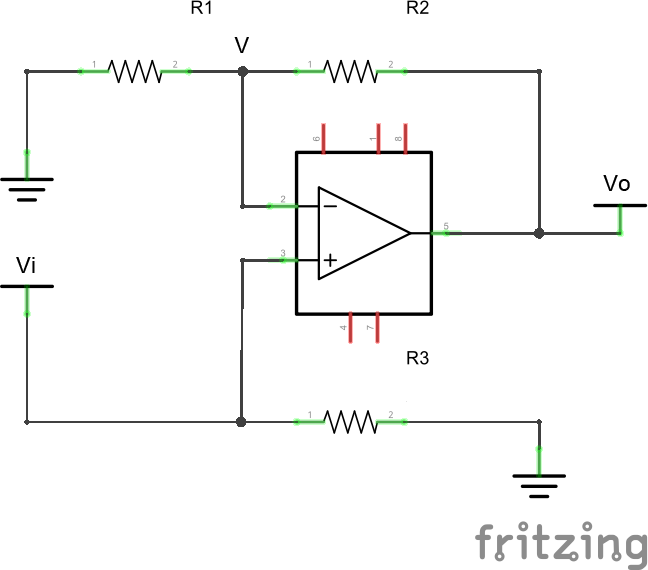
\includegraphics[width=0.8\textwidth]{figs/rel2/ex2.png}
    \caption{Circuito a ser analisado nos exercícios 2 a 4}
\end{figure}

Para obter a função de transferência do circuito descrito na figura 2, basta analisar a saída do amplificador operacional:
$$ V_o = \frac{A_0}{1+s \omega_b}(V_i-V) $$
Para descobrir $V$, vamos aplicar um divisor de tensão a partir de $V_o$:
$$ V = V_o \frac{R_1}{R_1 + R_2} $$
$$ \Rightarrow V_o = \frac{A_0}{1+s \omega_b} \left(V_i - V_o \frac{R_1}{R_1 + R_2} \right) $$
Isolando $V_o/V_i$ para obter a função de transferência,
$$ \Leftrightarrow \frac{V_o}{V_i} = \frac{A_o\cdotp(R_1 + R_2)}{s\cdotp\omega_b\cdotp(R_1+R_2)+R_1+R_2+A_oR_1} $$

\section{Exercício 3}

Pelo diagrama, nota-se que este é um circuito amplificador não-inversor. Neste caso, podemos utilizar a fórmula obtida em aula para a frequência de corte $f_c$:
$$ f_c = f_t \left( \frac{R_1}{R_1 + R_2} \right) $$

\section{Exercício 4}

% IDEA Check this: https://docs.scipy.org/doc/scipy/reference/generated/scipy.signal.bode.html
Utilizando os valores sugeridos para o experimento e a função de transferência obtida no exercício 2, podemos gerar os diagramas de Bode para o sistema numericamente. Os resultados estão nas figuras 3 e 4.

\begin{figure}
    \centering
    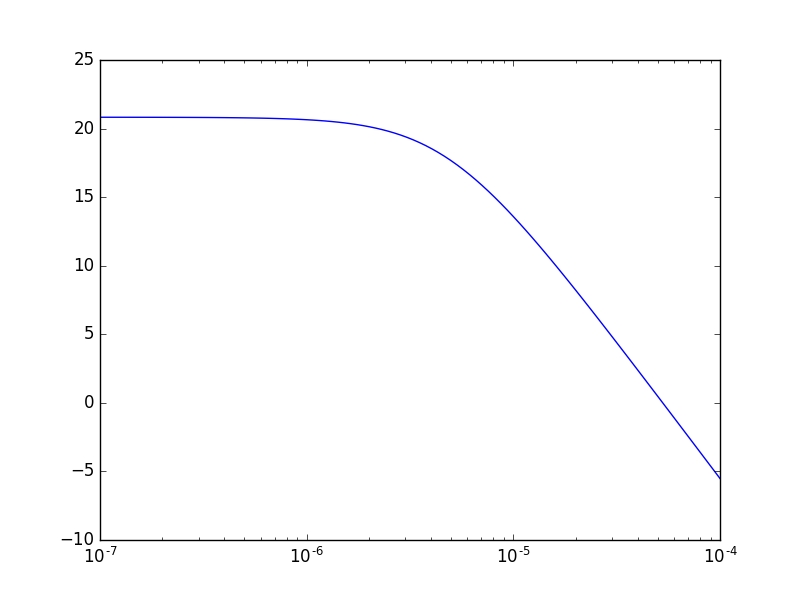
\includegraphics[width=0.8\textwidth]{figs/rel2/ex4-mag.png}
    \caption{Diagrama de Bode da magnitude}
\end{figure}

\begin{figure}
    \centering
    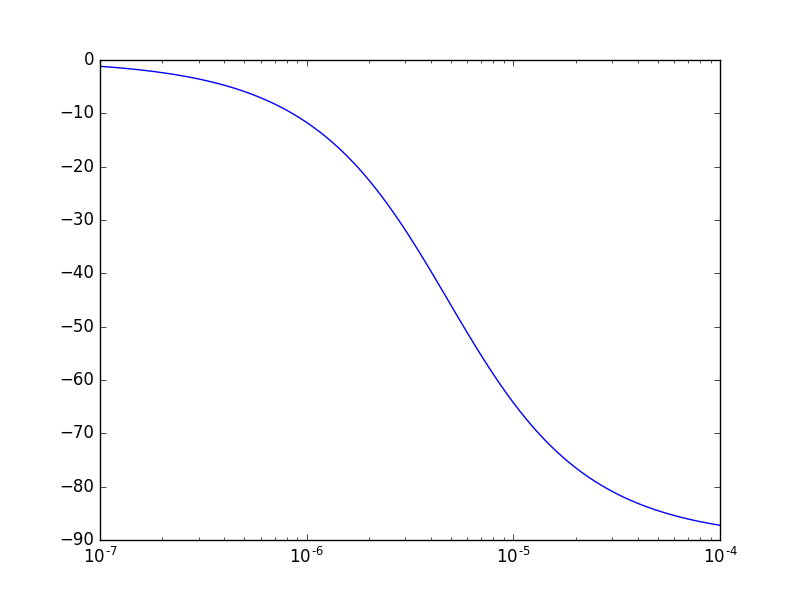
\includegraphics[width=0.8\textwidth]{figs/rel2/ex4-phase.png}
    \caption{Diagrama de Bode da fase}
\end{figure}

\section{Referência Bibliográfica}

\begin{itemize}
    \item Apostila do professor Humberto. http://paginapessoal.utfpr.edu.br/humberto/atividade-de-ensino/inicio/labeltronica. Acesso em 14 de Agosto de 2017.
    \item \textit{Datasheet} da família $TL074$. http://www.ti.com/lit/gpn/TL074. Acesso em 12 de Setembro de 2017.
    \item Notas de aula do professor Geovanny.
\end{itemize}

\end{document}
